\chapter{System Under Consideration} \label{ch:system}
The following chapter gives a thorough explanation of the system under consideration of this thesis. The system in question is the \textit{SecuritasHome startpaket}, which is a home alarm system from Securitas. This starter-kit includes multiple hardware components, as well as access to software portals and mobile applications to control the system.

\section{The companies behind the system}
This section covers the structure of the three major companies behind the SecuritasHome Home Alarm System.

While the system is sold and is branded by SecuritasHome, they actually have little to do with the actual hardware and software components of the platform, see figure \ref{fig:company-structure}. The hardware, related firmware, and proprietary radio wave protocol for communication between the components are manufactured and produced by a Taiwanese company called \textit{Climax Technology}. They are a major manufacturer of wireless home security systems. They produce hardware for home consumer security, creating everything from smart home alarm systems, and smart garage door openers, to smart medical accessories for seniors. The software, like the web portal and mobile applications as well as some additional firmware, are developed by an American company called \textit{Alarm.com}. They are strictly a B2B (business to business) company, meaning they do not sell or advertise their product directly to consumers. Instead they outsource the sale and advertisement of the system to other companies, one of them being Securitas. SecuritasHome merely sell, advertise, and put their brand on the product. Their main contribution to the system is in terms of real-time response to an alarm, connection to an alarm-central, and sending security personnel to respond to an active alarm breach. Consequently, when considering the cybersecurity of the system, Securitas is not strictly relevant. The two relevant parties are \textit{Alarm.com} and, considering the focus of this thesis, especially \textit{Climax Technology}.
\begin{figure}[!ht]
    \centering
    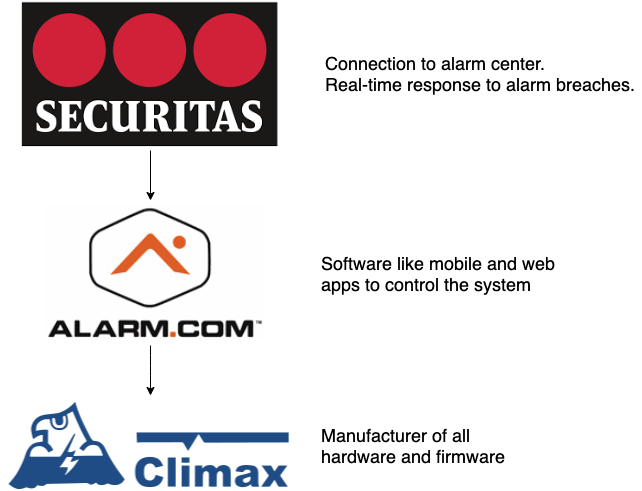
\includegraphics[width=0.7\textwidth]{images/company-structure.png}
    \caption{The companies behind the system.}
    \label{fig:company-structure}
\end{figure}

\section{Components and Software} \label{ch:system:components}
This section describes all the components and software of the system. Initially, all hardware components are described and their functionality. Lastly, all software components of the system are described. Note that the system supports many additional hardware components. The ones outlined below are only the ones part of the starter-kit.

\subsection{Hardware components} \label{ch:system:hardware}
The SecuritasHome starter-kit contains five hardware components, see figure \ref{fig:hardware-components}. These are described below. Note that the system supports many additional components, like smart locks for example. However, only the components included in the starter-kit are covered in this thesis.
\begin{figure}[!ht]
    \centering
    \begin{subfigure}[t]{0.33\textwidth}
        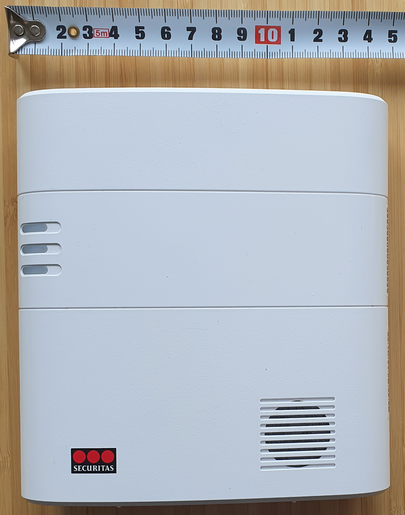
\includegraphics[height=2.15in]{images/main-panel.png}
        \caption{Main Panel}
        \label{fig:main-panel}
    \end{subfigure}%
    ~
    \begin{subfigure}[t]{0.33\textwidth}
        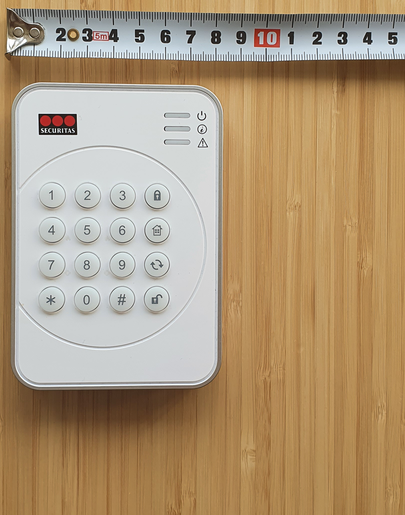
\includegraphics[height=2.15in]{images/keypad.png}
        \caption{Remote Keypad}
        \label{fig:remote-keypad}
    \end{subfigure}%
    ~
    \begin{subfigure}[t]{0.33\textwidth}
        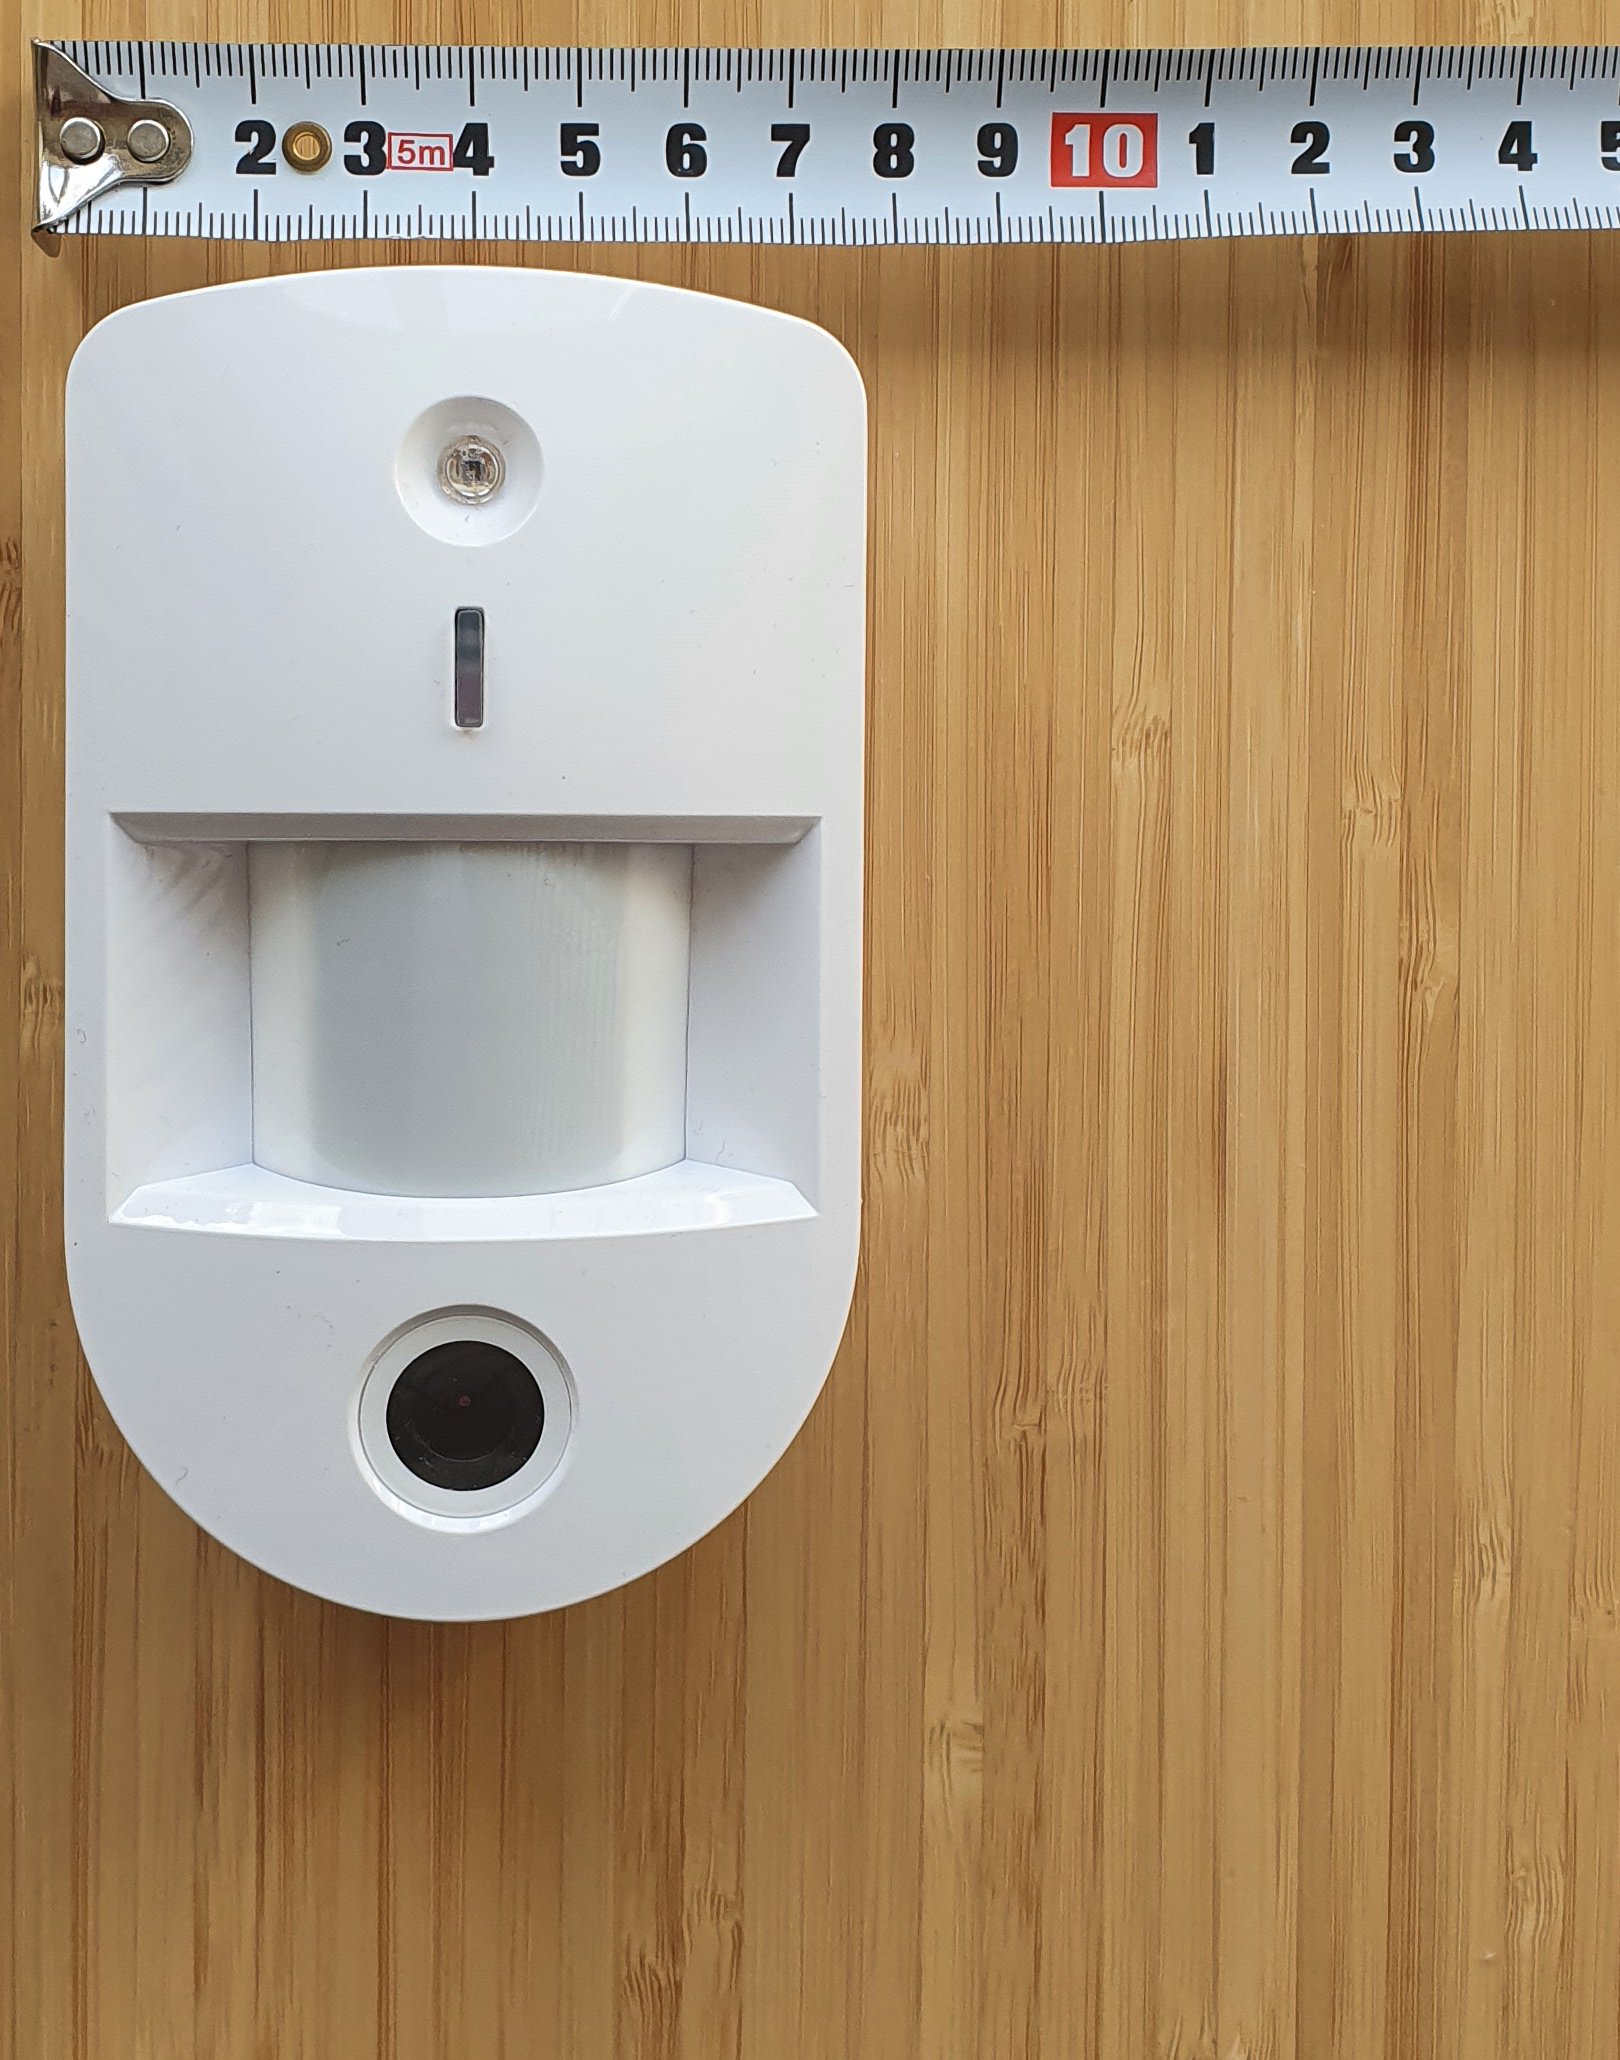
\includegraphics[height=2.15in]{images/camera.png}
        \caption{Motion Detection Camera}
        \label{fig:motion-camera}
    \end{subfigure}
    
    \begin{subfigure}[t]{0.33\textwidth}
        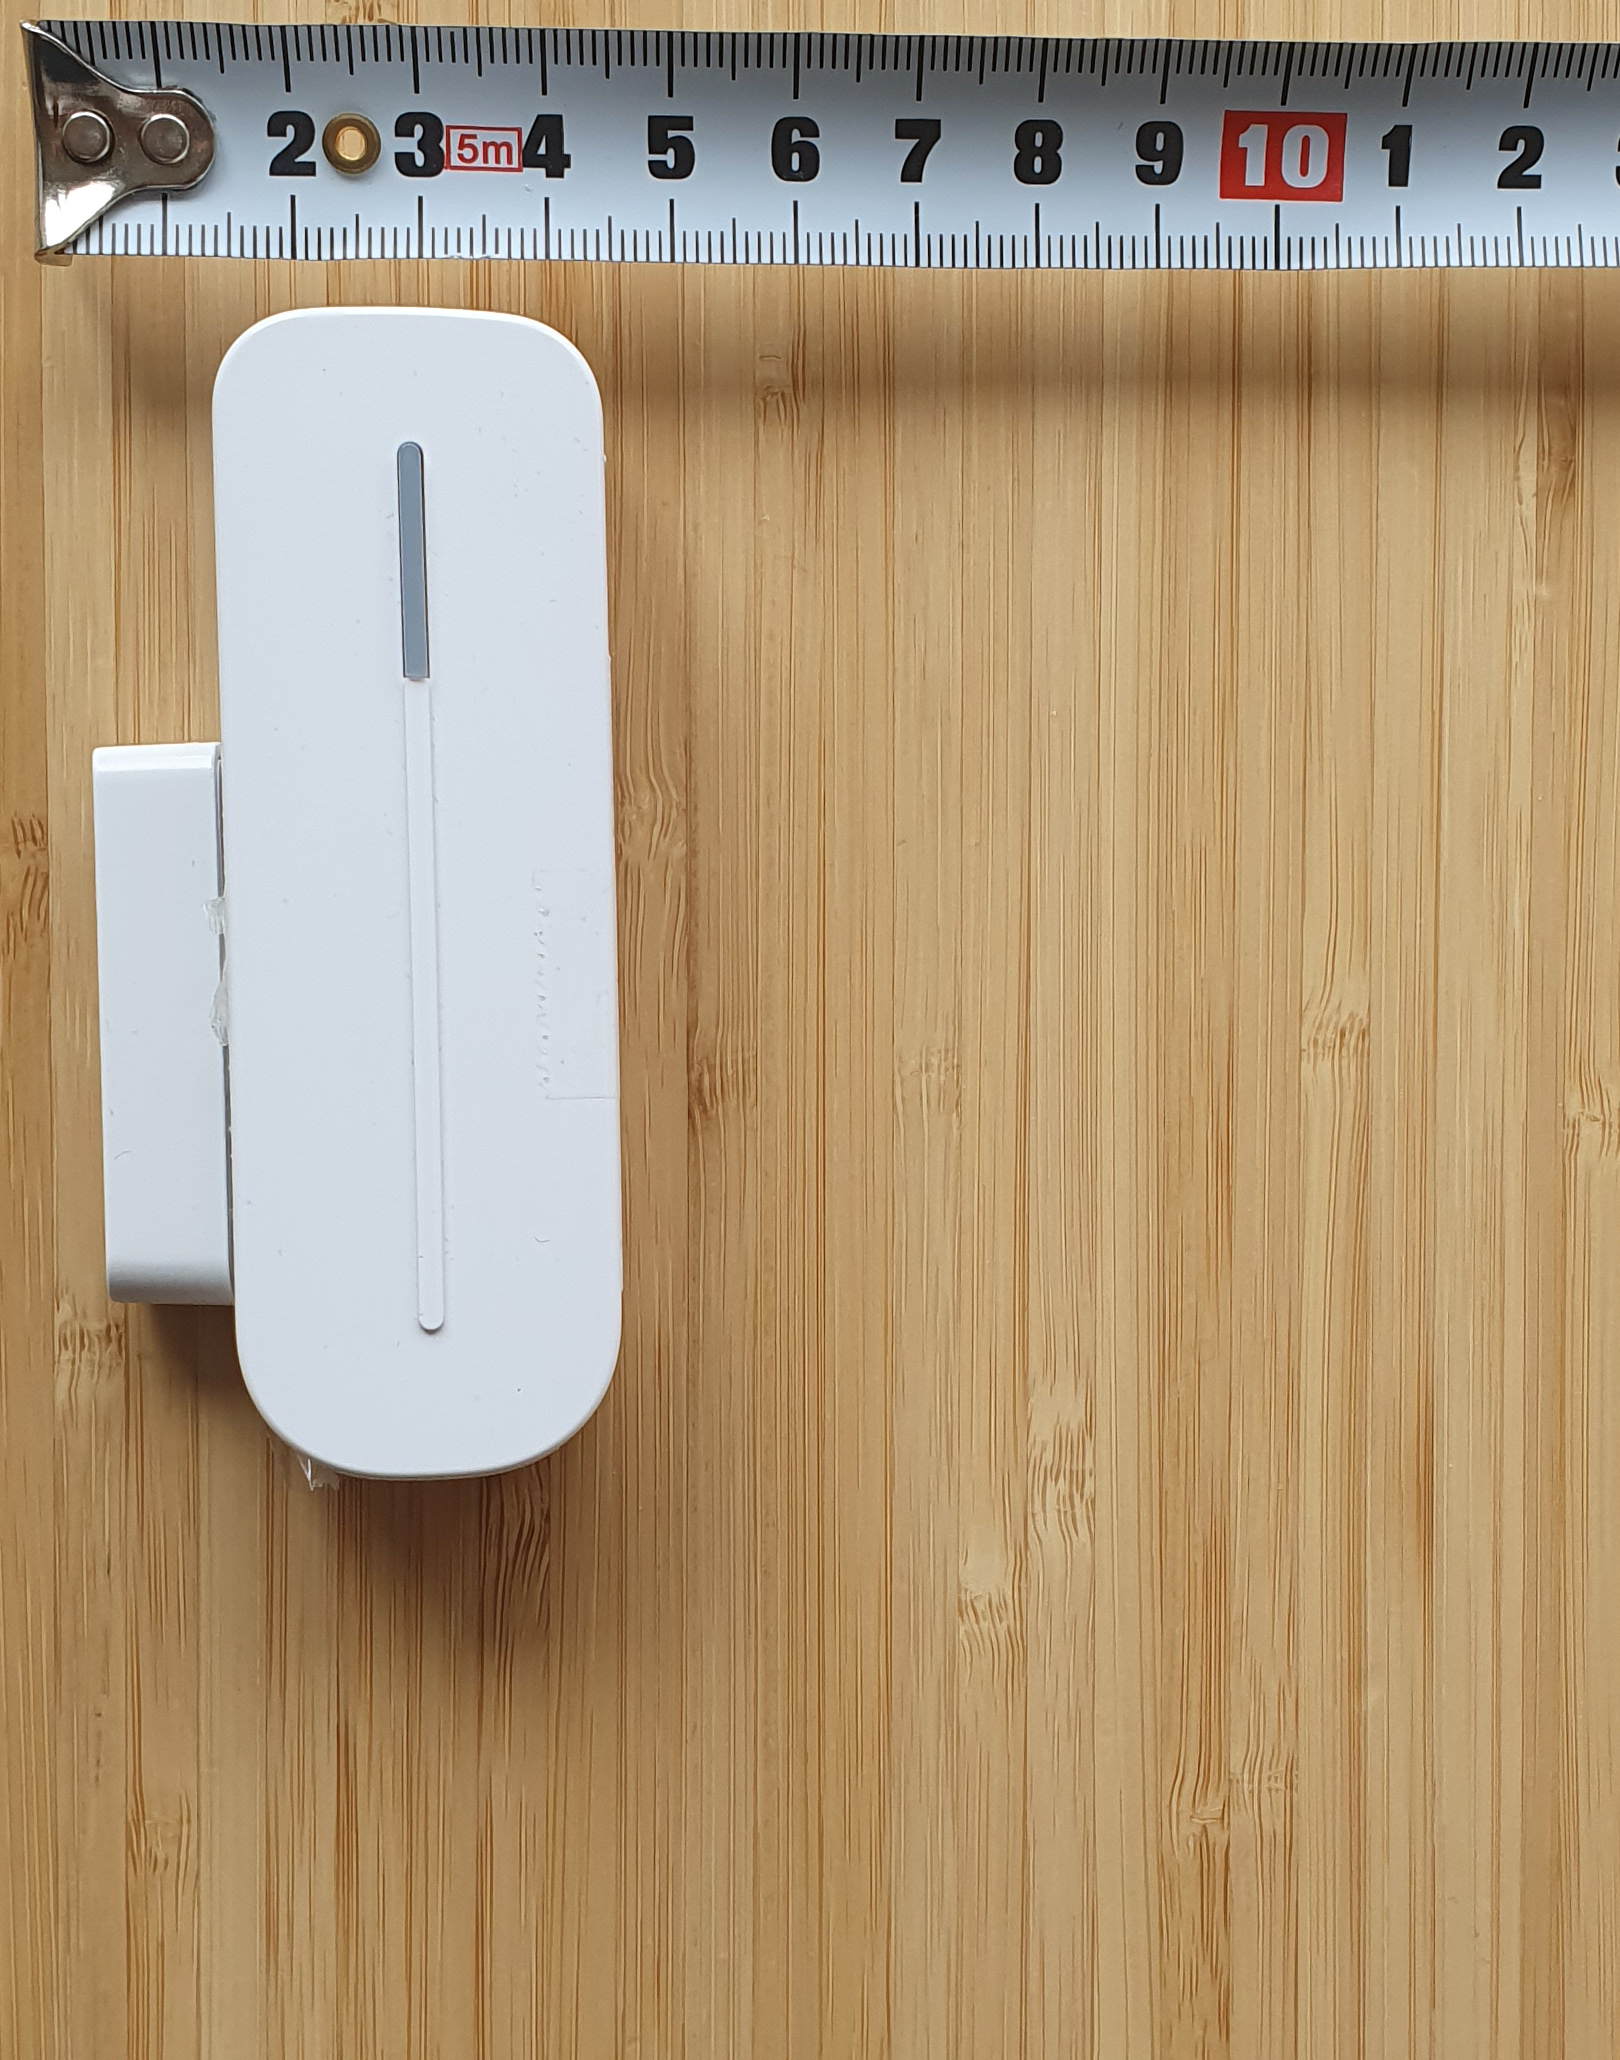
\includegraphics[height=2.15in]{images/door-contact.png}
        \caption{Door Contact Sensor}
        \label{fig:door-contact}
    \end{subfigure}%
    ~
    \begin{subfigure}[t]{0.33\textwidth}
        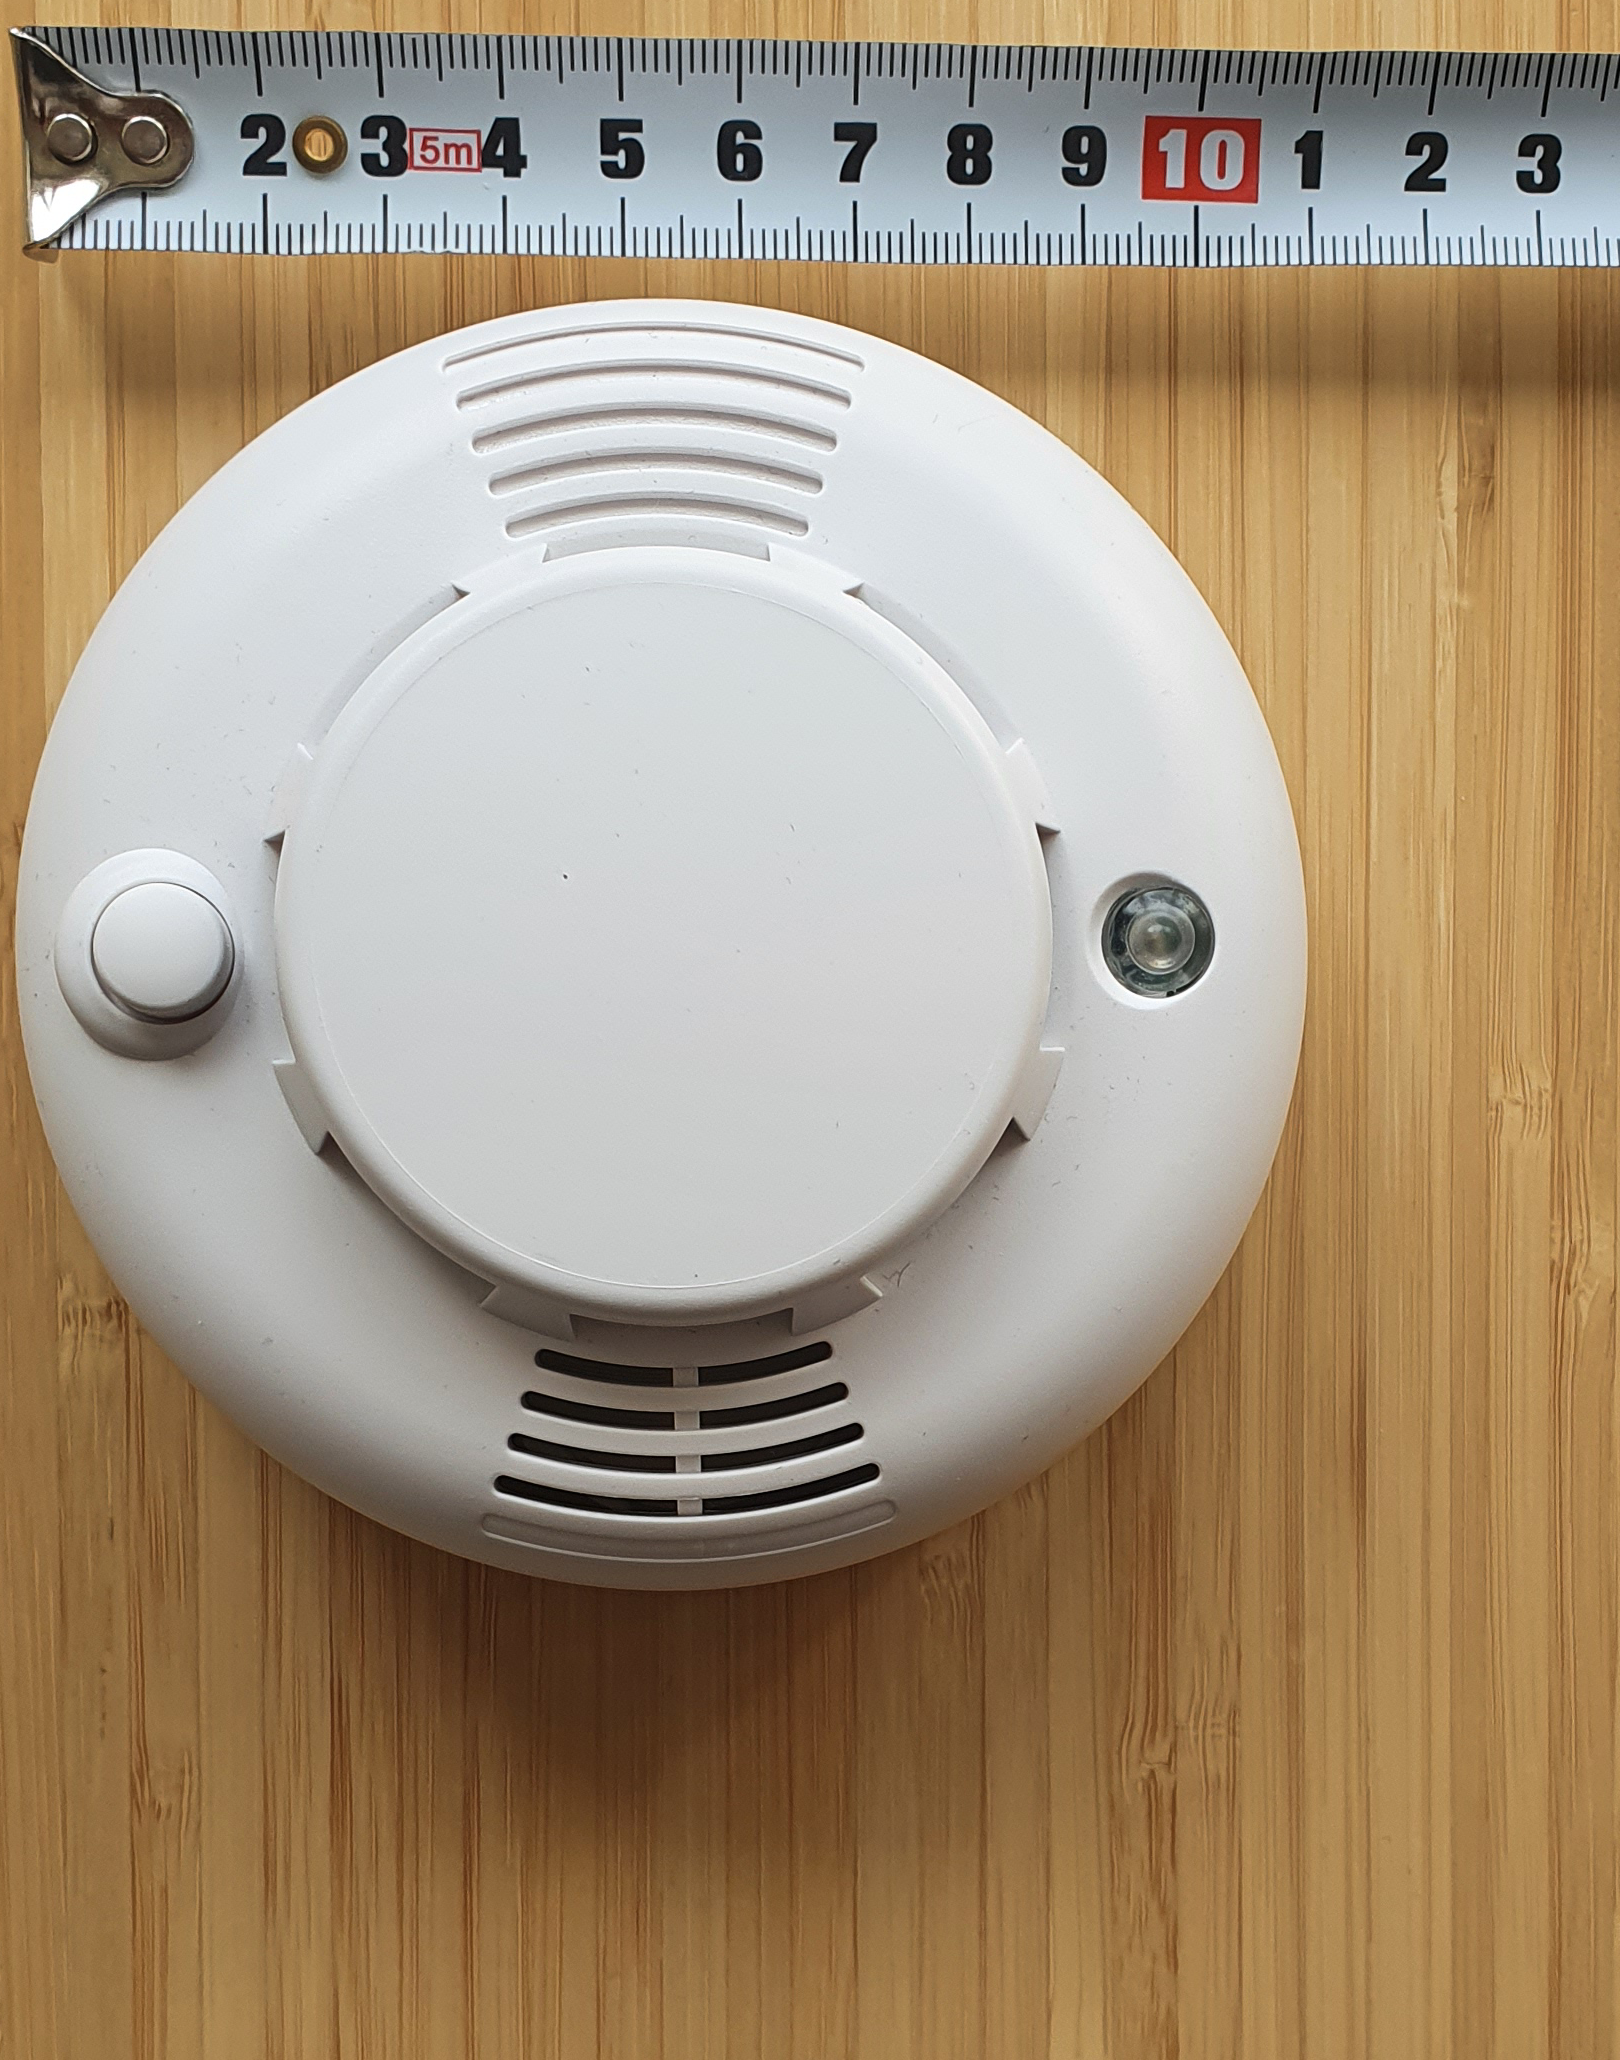
\includegraphics[height=2.15in]{images/smoke-detector.png}
        \caption{Smoke Detector}
        \label{fig:smoke-detector}
    \end{subfigure}
    \caption{The hardware components of the system}
    \label{fig:hardware-components}
\end{figure}
\subsubsection{Main Panel}
\textbf{Model number:} HSGW-G8-3G/LTE-ZW-F1 433/868 \\
\textbf{FCCID:} GX9HSGWF1919 \\
The main panel, see figure \ref{fig:main-panel}, is the \textit{"brains"} of the system so to speak. It handles communication with all other hardware devices as well as external servers. Through radio wave communication it talks to the other hardware peripherals of the system. It uses 3G telecommunication to talk to the external servers.

\subsubsection{Remote Keypad}
\textbf{Model number:} KPT-23-EL-F1 \\ % could also be KPT-23N-EL-F1, not sure
\textbf{FCCID:} GX9KPF1 \\ % This says KPF but it looks the same..
The remote keypad is a 16 button keypad used to arm and disarm the system using a personal 4 digit pin. See figure \ref{fig:remote-keypad}. This device talks to the main panel over radiowave communication.

\subsubsection{Motion Detection Camera}
\textbf{Model number:} VST-862-F1 \\
\textbf{FCCID:} GX9862 \\
This device, see figure \ref{fig:motion-camera}, features an infra-red sensor to detect motion, and a camera to survey the location. When triggered the device takes two pictures which are sent to the main panel. It is not a surveillance camera, meaning it does not continuously take pictures. The camera is only active when motion is detected and the alarm is triggered, presumably to save power.

\subsubsection{Door Contact Sensor}
\textbf{Model number:} DC-23-F1 \\
\textbf{FCCID:} GX9DC23 \\
This device, see figure \ref{fig:door-contact}, senses when a door or window is opened. A small external magnet is placed on the door/window close to the device. When these are separated the device is triggered and communicates with the main panel over radio wave communication.

\subsubsection{Smoke Detector}
\textbf{Model number:} SD-8EL \\
\textbf{FCCID:} GX9SD8ELF1919 \\
This device is a smoke detector, see figure \ref{fig:smoke-detector}. It communicated with the main panel over radio-waves and also includes a siren which triggers when it detects smoke.

\subsection{Software} \label{ch:system:software}
This section details the three software entry points from where the user can control the alarm and view it's state.

\subsubsection{Web portal}
The web portal is a webpage created by the American company \textit{Alarm.com}, see figure \ref{fig:company-structure}, hosted at \url{https://www.alarm.com/web/system/}. From the landing page, see figure \ref{fig:web-landing-page}, the user see the following:
\begin{itemize}
    \item If the system has any issues. This can be seen in the \textit{System OK} box in figure \ref{fig:web-landing-page}.
    \item The state of each sensor of the system, like the door contact sensor (see figure \ref{fig:door-contact}).
    \item The arm/disarm state of the system.
\end{itemize}
Crucially, from the landing page, the user can also easily arm or disarm the system, see figure \ref{fig:web-arming}. Beyond this, the user can also see a list of recent activity in the system, change users personal four digit pin codes, and create new users.

\begin{figure}[!ht]
    \centering
    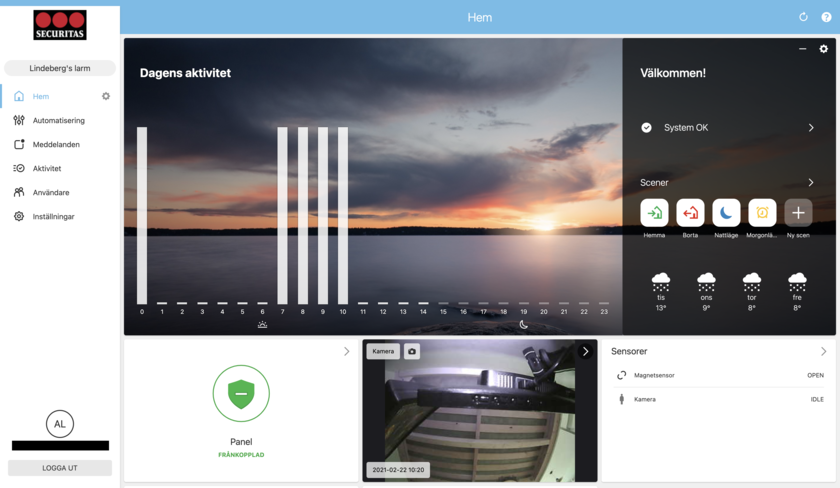
\includegraphics[width=\textwidth]{images/landing-page-web.png}
    \caption{The web portal landing page.}
    \label{fig:web-landing-page}
\end{figure}
\begin{figure}[!ht]
    \centering
    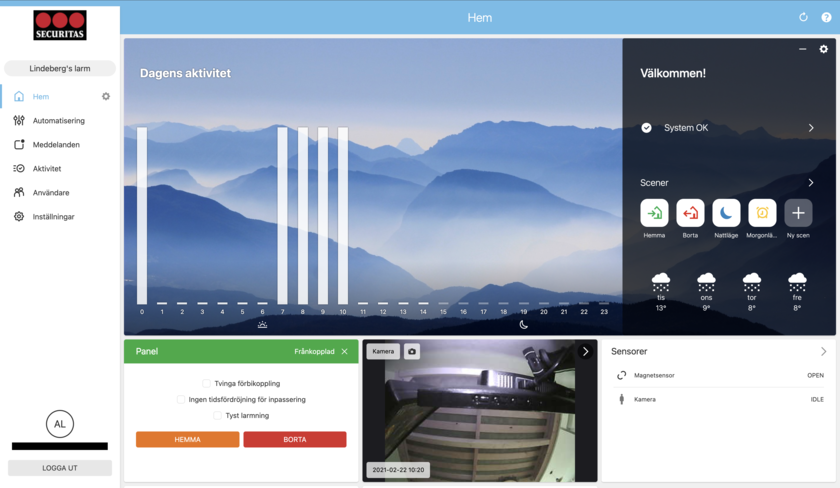
\includegraphics[width=\textwidth]{images/arming-web.png}
    \caption{Arming the alarm from the web portal.}
    \label{fig:web-arming}
\end{figure}

\subsubsection{Mobile application}
Note that only the \textit{Android} version of the mobile app is covered here, but presumably the iOS version would have similar or identical features.

The system can also be controlled and administrated via a mobile application, free to download via the \textit{Google Play Store}, called \textit{Securitas Connect}\footnotelink{https://play.google.com/store/apps/details?id=com.alarm.alarmmobile.android.securitas}{2021-03-30}. As explained previously, while the application is branded by Securitas, it is created and developed by \textit{Alarm.com}. The interface very closely resembles the web portal (see section above) and offers identical functionality, see figure \ref{fig:mobile-landing-page}.
\begin{figure}[!ht]
    \centering
    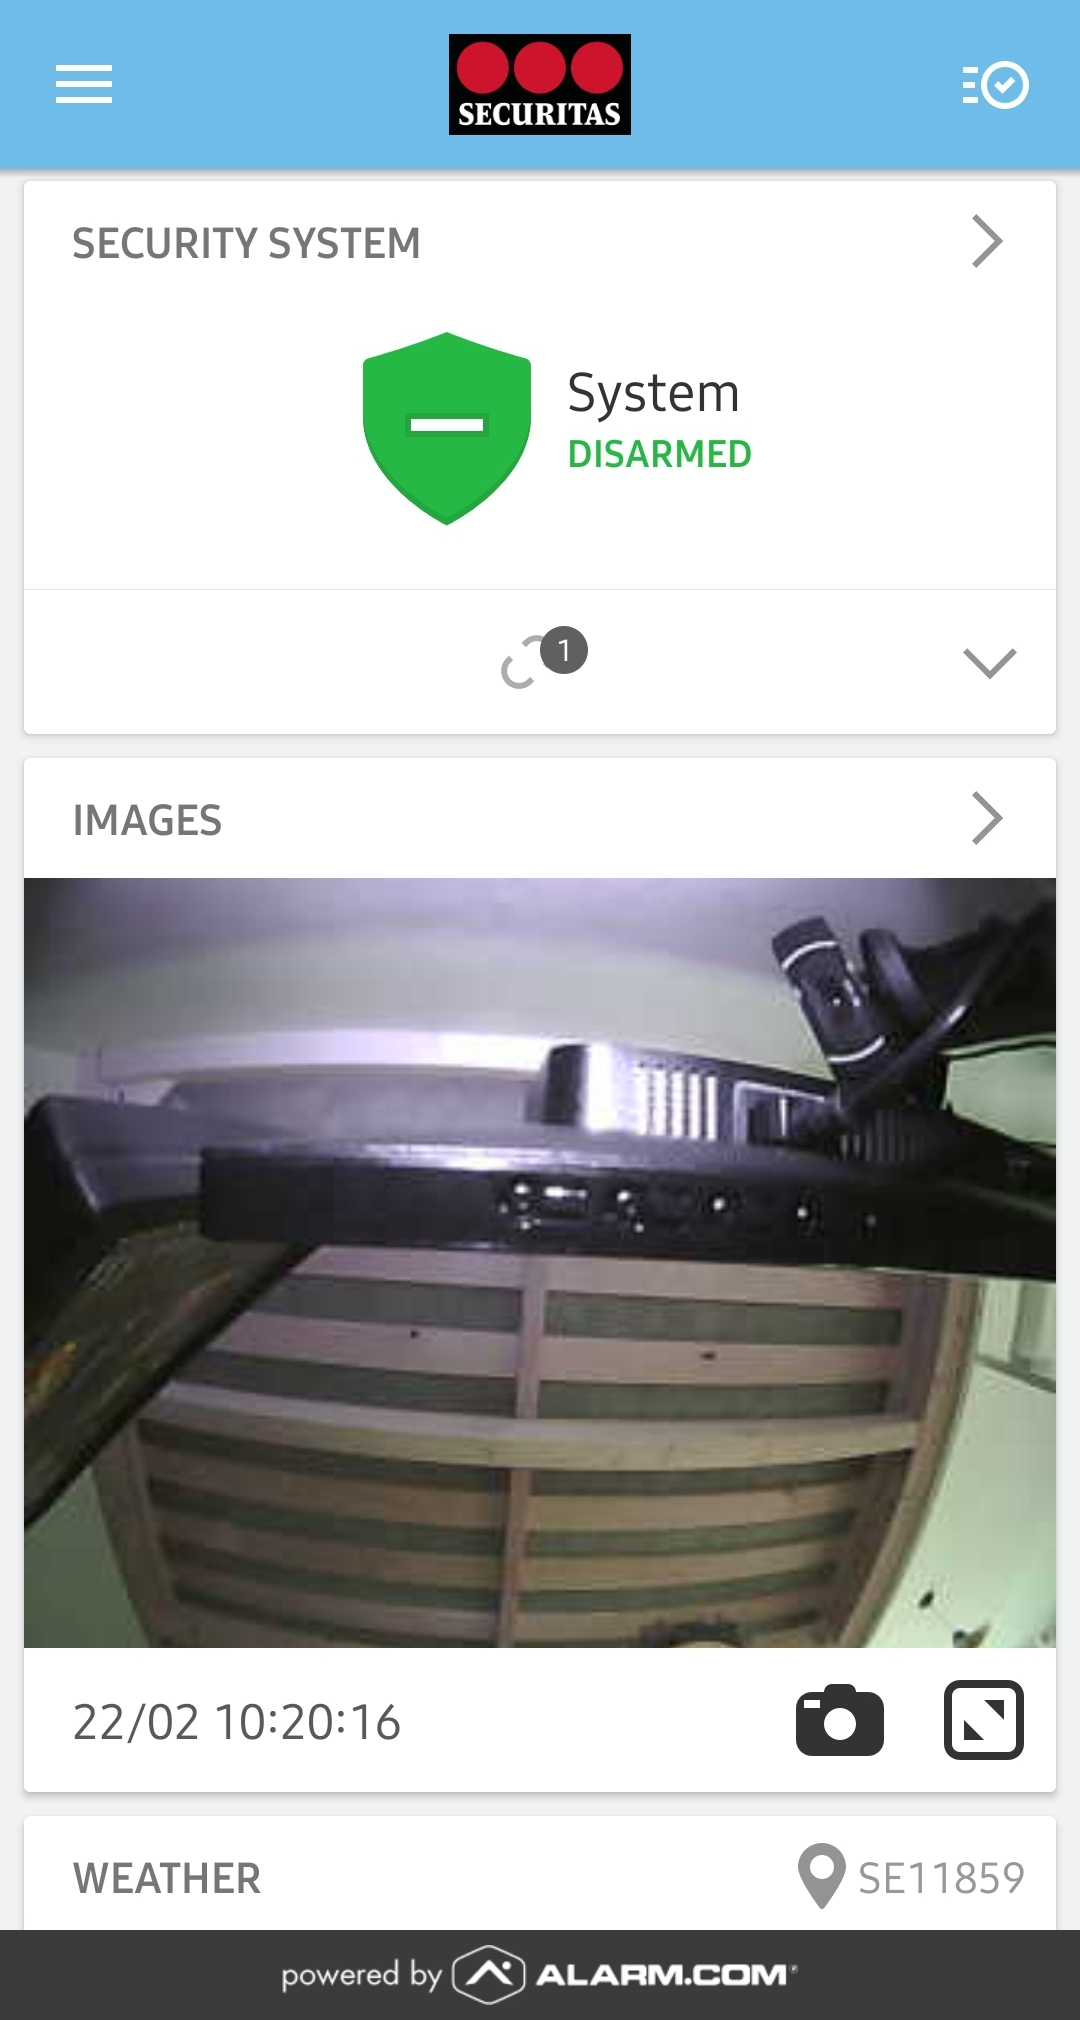
\includegraphics[width=0.5\textwidth]{images/mobile-landing-page.jpg}
    \caption{The android mobile app landing page.}
    \label{fig:mobile-landing-page}
\end{figure}

\subsubsection{Local web admin page}
Beyond the two applications created by \textit{Alarm.com} described above, the main panel (see figure \ref{fig:main-panel}) hosts a web server on the local network. This feature is undocumented, and is presumably not meant to be used or found by the regular, non-tech-savvy consumer. The page is not hosted on any domain name, as far as the author is aware, and instead has to be accessed directly via the main panels local IP address on port 80. The landing page of this web server is quite simple and shows some basic information about the system such as the MAC address, IMEI number of the cellular communication, etc., see figure \ref{fig:local-landing-page}. Beyond that, the site only has two actions the user can do. One is to perform a "\textit{Phone Test}", to presumably test the connection to the mobile 3G network, and the other is a "\textit{Network Scan}". Once the network scan has completed, the page shows a list of all reachable telecommunication towers, see figure \ref{fig:local-network-scan}.
\begin{figure}[!ht]
    \centering
    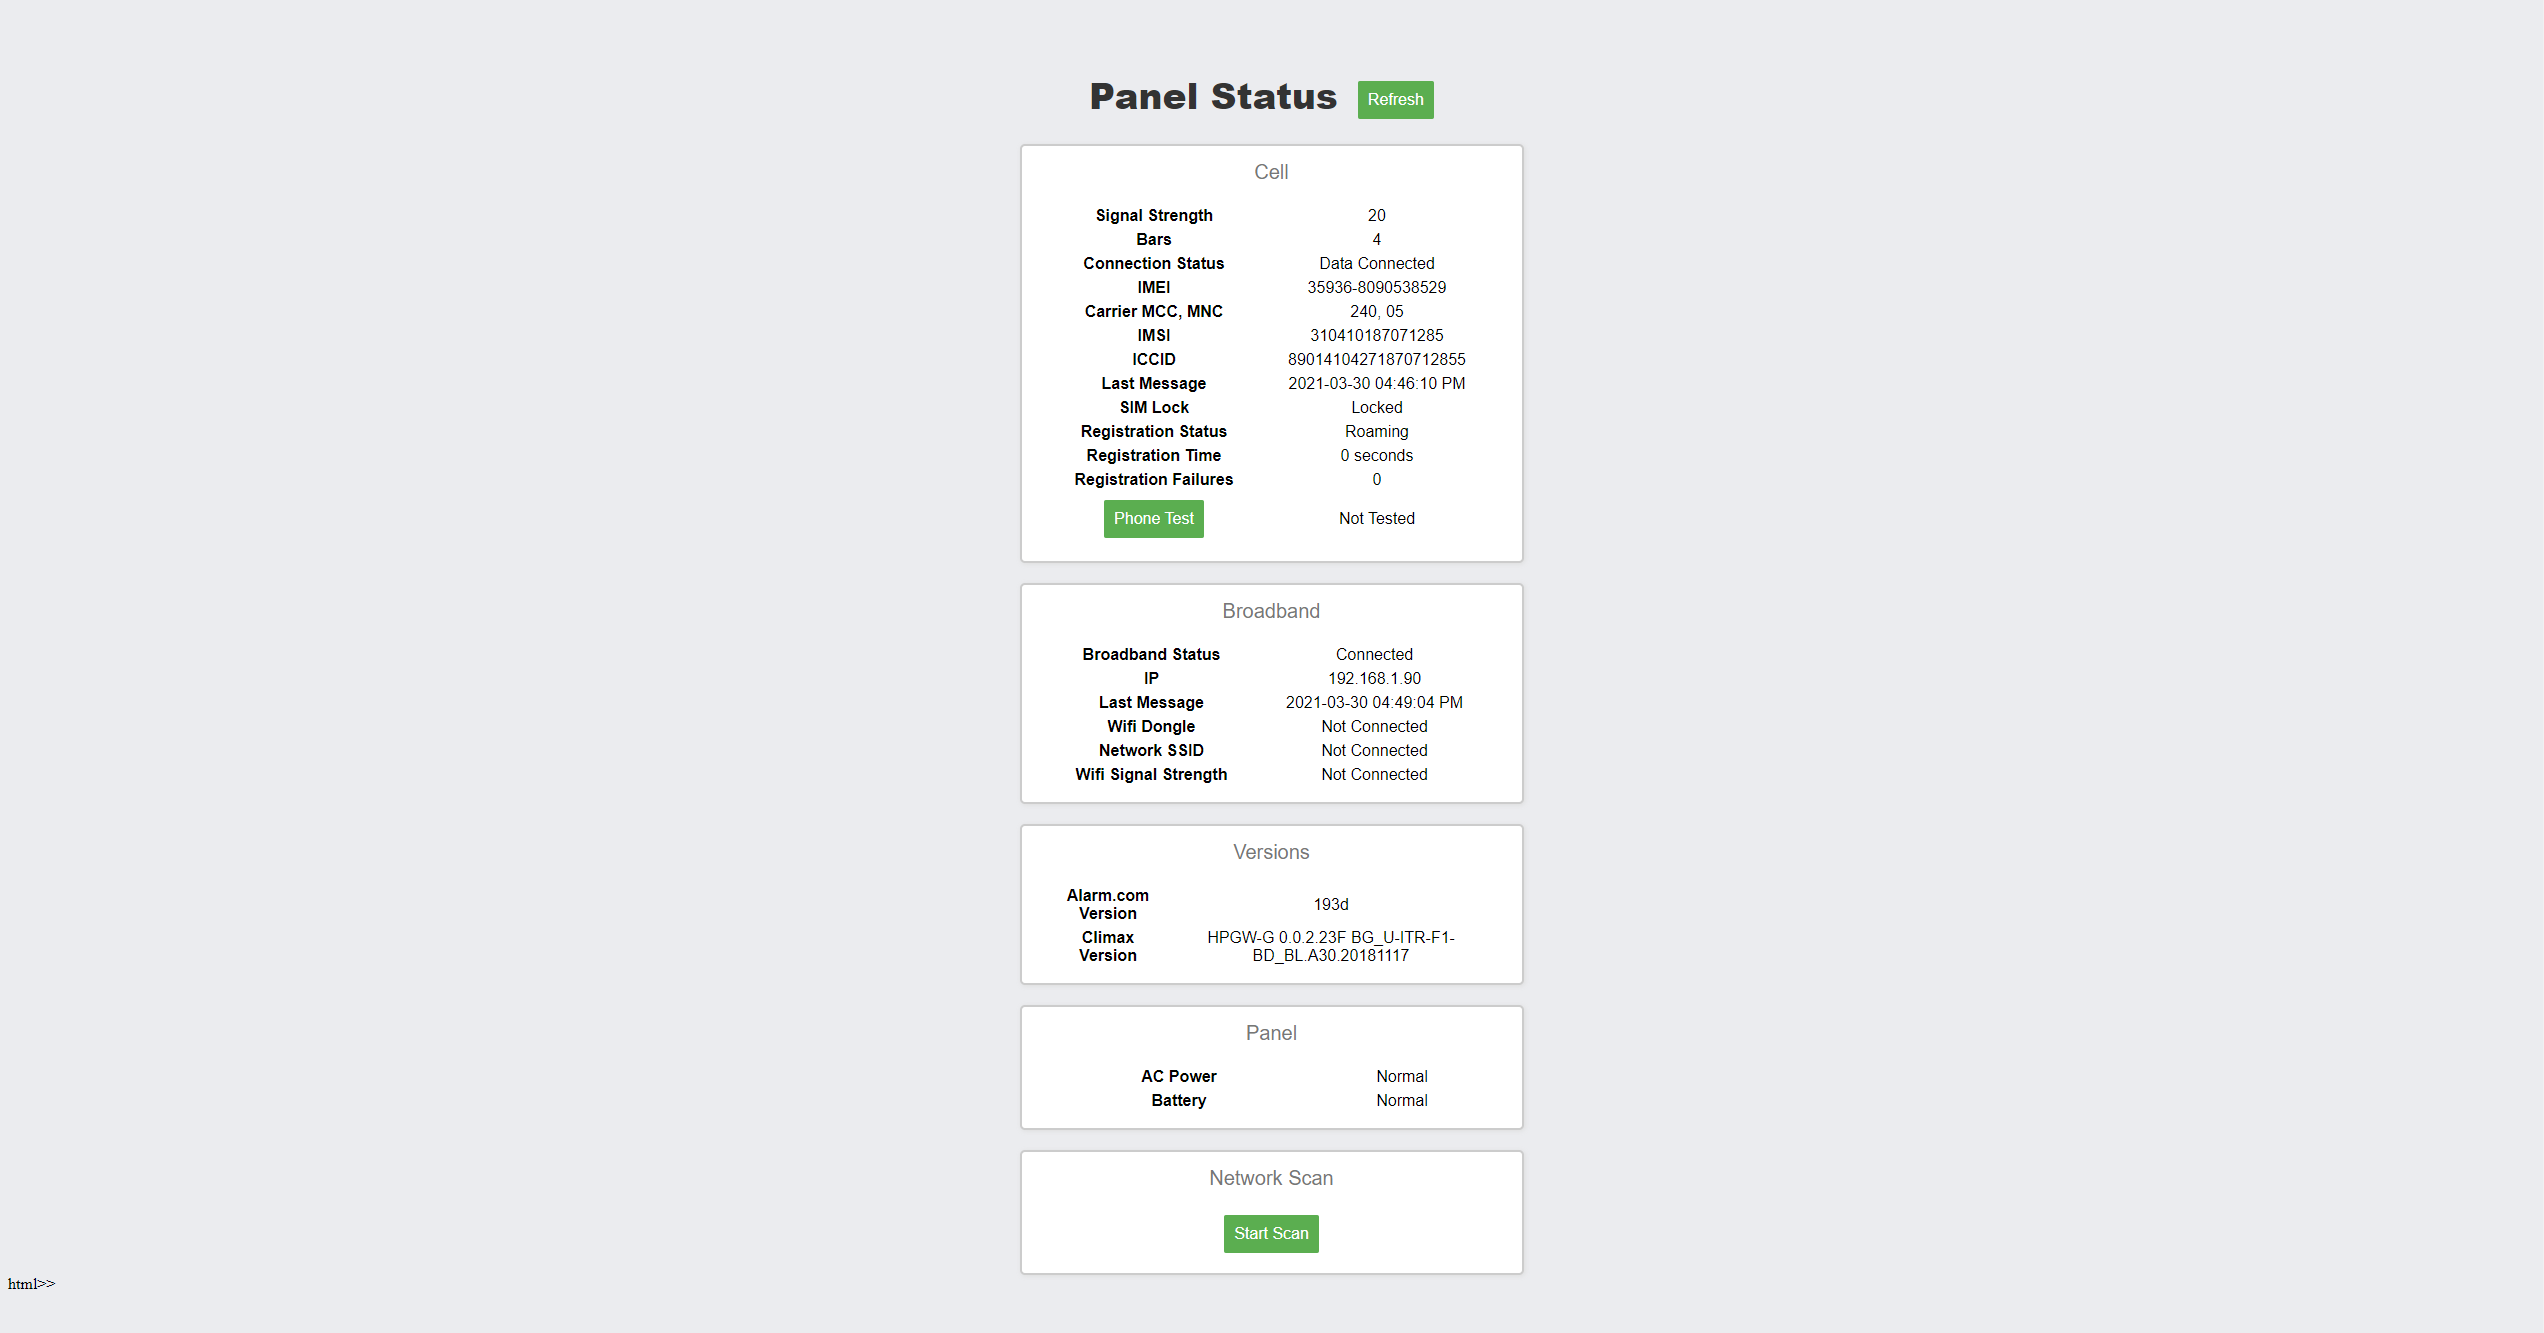
\includegraphics[width=\textwidth]{images/local-landing-page.png}
    \caption{The local web server's landing page.}
    \label{fig:local-landing-page}
\end{figure}
\begin{figure}[!ht]
    \centering
    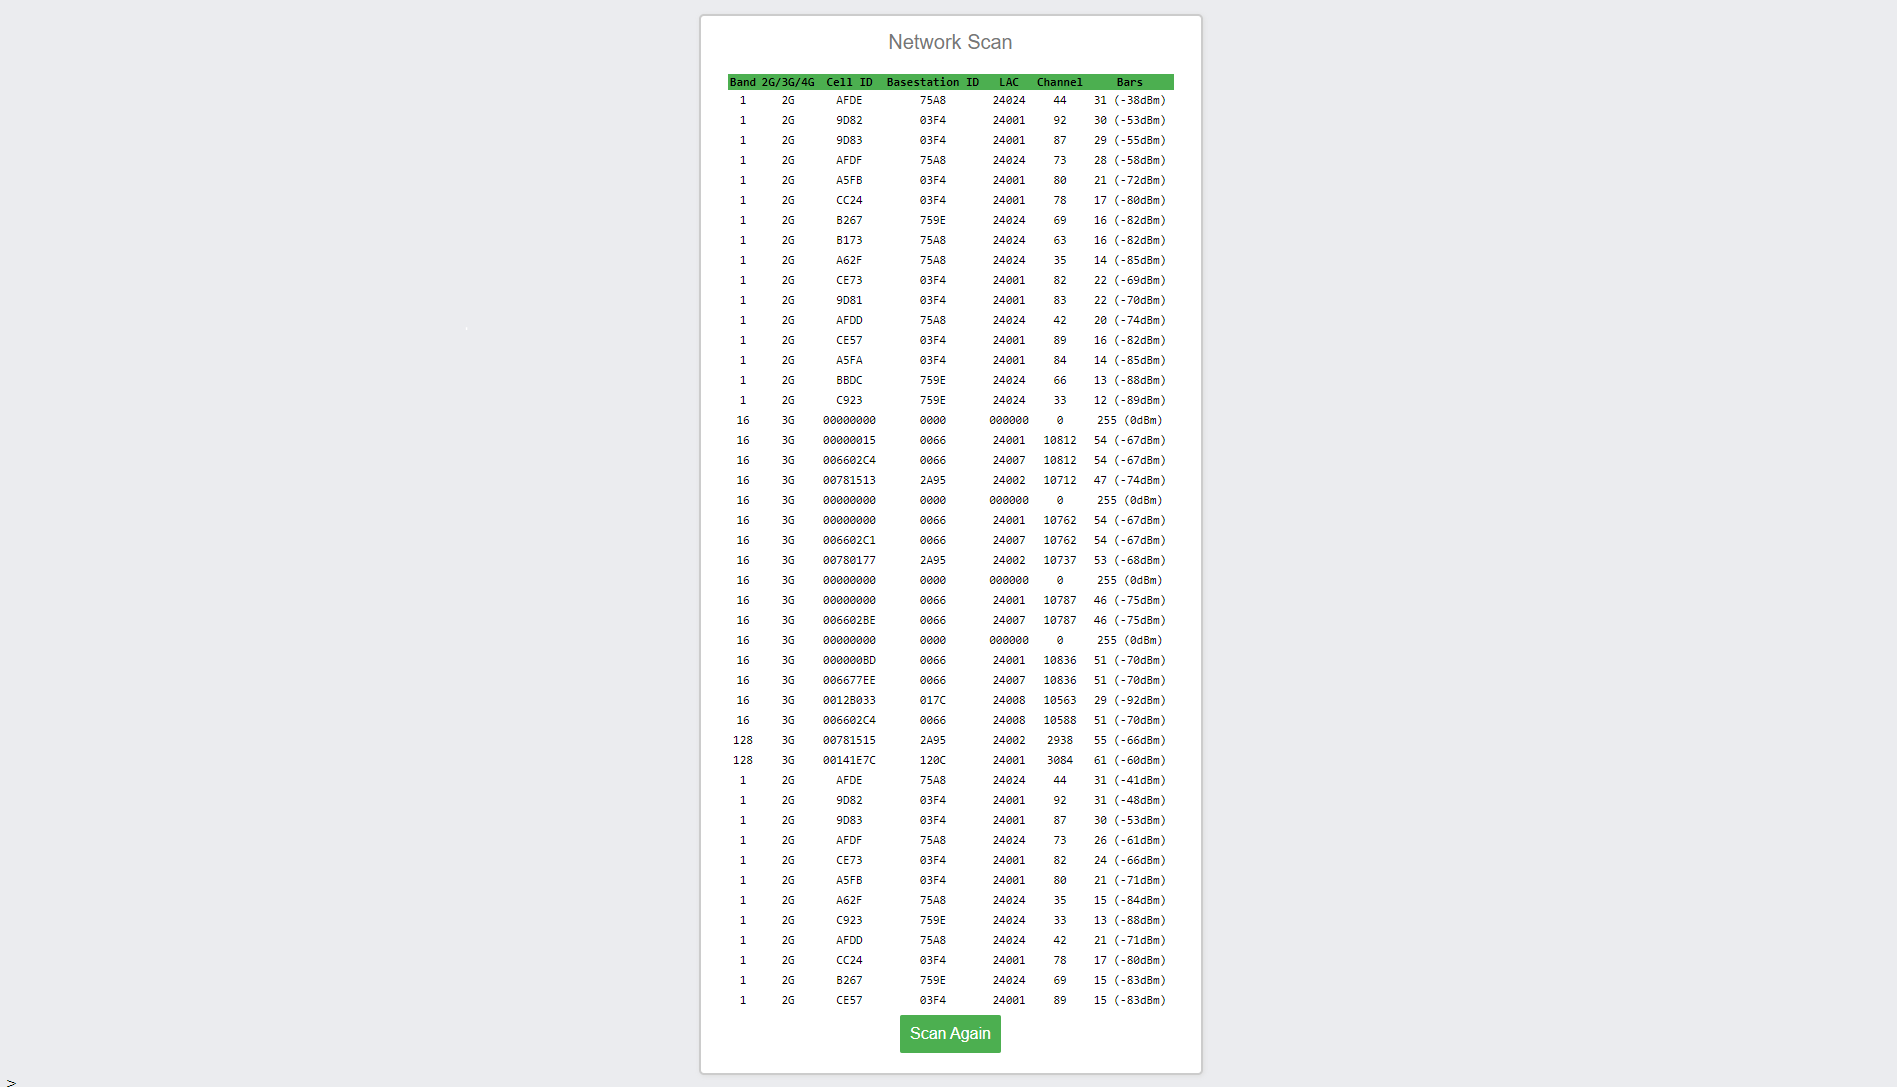
\includegraphics[width=\textwidth]{images/local-network-scan.png}
    \caption{A mobile network scan from the local web server.}
    \label{fig:local-network-scan}
\end{figure}
Additionally, the web page features a login page on the path \texttt{/action/login} which lets the user authenticate using \textit{HTTP Basic auth}. The credentials here are not tied to the users account, so presumably this is purely meant as a backdoor for \textit{Climax Technology} for debugging purposes, and not meant to be used by the user of the system.